\documentclass{article}

\usepackage{setspace}
\usepackage[utf8]{inputenc}
\usepackage{amsmath}
\usepackage{amsthm}
\usepackage[colorlinks]{hyperref}
\hypersetup{%
    colorlinks=true,
    linkcolor=blue,
    urlcolor=cyan,
    citecolor=blue
}
\usepackage[inline]{enumitem}
\usepackage{mathtools}
\newlist{inlist}{enumerate*}{1}
\setlist[inlist]{label= (\alph*)}
\usepackage{booktabs}
\usepackage{multirow}
\usepackage{graphicx}
\usepackage{smartdiagram}
\usepackage{subcaption}
\usepackage{float}
\floatstyle{boxed}
\restylefloat{figure}
\restylefloat{table}
\usepackage{biblatex}
\addbibresource{sources.bib}
\usepackage[nopostdot,toc,acronym,nomain,nonumberlist]{glossaries}
{\makeglossaries}
\loadglsentries[acronym]{glossary}
\usepackage{tikz}
\usetikzlibrary{shapes,positioning,arrows,calc}

\newcommand{\mylongtitle}{MS Report \\
On the state of verified programs research}
\newcommand{\mysubtitle}{}
\newcommand{\myshorttitle}{}
\newcommand{\mytitle}{\mylongtitle}

% Preamble {{{

% newcommands, DeclareMathOperators, &c. {{{
\theoremstyle{plain} % default
\newtheorem{thm}{Theorem}[section]
\newtheorem{lem}[thm]{Lemma}
\newtheorem{prop}[thm]{Property}
\newtheorem*{cor}{Corollary}

\theoremstyle{definition}
\newtheorem{defn}{Definition}[section]
\newtheorem{example}{Example}[section]
\newtheorem{exercise}{Exercise}[section]
\newtheorem*{prob}{Problem}

\theoremstyle{remark}
\newtheorem*{rem}{Remark}
\newtheorem*{note}{Note}
\newtheorem{case}{Case}

\newcommand{\yields}{\Rightarrow}
\newcommand{\Yields}{\Rightarrow^{\star}}
\newcommand{\union}{\cup}
\newcommand{\intersect}{\cap}
\newcommand{\Union}{\bigcup}
\newcommand{\Intersect}{\bigcap}
\newcommand{\compose}{\mathrel{\circ}}
\newcommand{\setcompl}[1]{{\overline{#1}}}
\newcommand{\DownTo}{\mathrel{\Downarrow}}
\newcommand{\To}{\mathrel{\Rightarrow}}
\newcommand{\TO}{\mathrel{\Rrightarrow}}
\newcommand{\definedas}{\triangleq}
\newcommand{\matches}{\mathrel{\cong}}

\newcommand{\bb}[1]{\mathbb{#1}}
\newcommand{\N}{\bb{N}}
\newcommand{\Z}{\bb{Z}}
\newcommand{\Q}{\bb{Q}}
\newcommand{\R}{\bb{R}}
\newcommand{\I}{\bb{I}}

\newcommand{\mc}[1]{\mathcal{#1}}
\newcommand{\Powerset}[1]{\mc{P}\left(#1\right)}

\newcommand{\set}[1]{\left\{#1\right\}}
\newcommand{\setbuild}[2]{\left\{ #1 : #2\right\}}

\newcommand{\var}[1]{\mathit{#1}}
\newcommand{\func}[1]{\mathsf{#1}}
\newcommand{\iname}[1]{\textsf{#1}}

\DeclareMathOperator{\false}{false}
\DeclareMathOperator{\true}{true}

\DeclarePairedDelimiter{\abs}{\lvert}{\rvert}
\DeclarePairedDelimiter{\norm}{\lVert}{\rVert}
\DeclarePairedDelimiter{\ceil}{\lceil}{\rceil}
\DeclarePairedDelimiter{\floor}{\lfloor}{\rfloor}
\DeclarePairedDelimiter{\denote}{\llbracket}{\rrbracket}

\DeclareMathOperator{\lcm}{lcm}

\newcommand{\wpre}[1]{\func{wp}\denote{#1}}

\newcommand{\idem}{\emph{idem.}}
\newcommand{\vs}{{\emph{v{.}}}}
\newcommand{\ie}{\emph{i.e.}}
\newcommand{\eg}{\emph{e.g.}}
\newcommand{\etc}{\emph{etc.}}
\newcommand{\etal}{\emph{et al.}}

\newcommand{\haltprob}{\emph{Entscheidungsproblem}}
% newcommands, DeclareMathOperators, &c. }}}

% Preamble }}}


\begin{document}

\title{\mytitle}
\author{D. Ben Knoble \\
Department of Computer Science \\
University of North Carolina at Chapel Hill}
\date{April 2020}

\maketitle

\begin{abstract}
    This report explores the current state of verified programs research through
several lenses. We begin with a historical background of formal methods before
switching to formal verification in modern programming environments. In
particular, we examine verified user-programs and compilers. Next we categorize
verified programming tools along three (3) axes:
\begin{inlist}
\item interactivity,
\item proof logic, and
\item programming language.
\end{inlist}
Following that, we compare two extended examples of verified programs in
different systems. We also discuss a number of modern research projects and the
impacts they have had on formal verification, especially at scale and in
security-related settings. Lastly, we summarize the challenges of formal
verification in today's settings: notably, these include scaling proofs,
automation and proof management, symbolic explosion, and cross-language
verification. We conclude with a reminder that formal verification is another
tool in the programmer's toolbox and that the programmer must exercise
appropriate judgement in deciding which tool will solve a given problem.

\end{abstract}

Approved by:

Primary reader: Don Porter {\hrulefill}

Secondary reader: Cynthia Sturton {\hrulefill}

\begin{singlespace}
    \newpage
    \tableofcontents

    \newpage
    \listoffigures
    \listoftables
\end{singlespace}

\newpage

\glsresetall[acronym]

\section{Introduction}

First, we introduce the ideas of formal methods and formal verification, in
particular their connection to programming. Next, we briefly dissect the various
layers of abstraction that programmers operate in and the corresponding
layers of verification. Finally, we outline the direction of the rest of this
report.

\subsection{Background}\label{S:background}

Formal methods are mathematical techniques for describing and verifying system
properties~\cite{Wing_90}. They have been successfully applied to the practice
of programming and computation since the birth of computing:
\citeauthor{Turing_1937}'s famous 1937 discussion of the {\haltprob} is an
application of mathematical reasoning to a generalized system of
computation~\cite{Turing_1937}. The use of formal methods continued throughout
the modern computing era, with \citeauthor{McCarthy_67} formalizing the first
proof of a verified compiler in 1967~\cite{McCarthy_67}. The proof was later
mechanically verified to be correct in 1972~\cite{Milner_72}. The computing
giant and prolific writer \citeauthor{EWD:EWD1036} argued in 1988 that the very
nature of programming depended on notions of symbolic manipulation, formal
semantics, and the task of giving a ``formal proof'' that the proposed program
``meets the equally formal functional specification''---and that Computer
Science education at the time generally omitted much of the relevant background
and material necessary for accomplishing this task~\cite{EWD:EWD1036}.

Formal verification, \citeauthor{EWD:EWD1036}'s act of proving that the program
implements its specification, has not died as he predicted through a ``foggy
crystal ball.'' Instead, formal methods have become increasingly powerful,
accessible, and vital, as we aim to elucidate here. Some computer scientists
hesitate to make claims about the termination of a particular
program~\cite{Cook_2011}, perhaps intimidated by \citeauthor{Turing_1937}'s
Halting Problem arguments; yet, proofs of termination, correctness,
non-interference, and more are increasingly necessary and useful to reason about
programs. For example, such proofs are now used to reason about \gls{os}
kernels~\cite{Klein_EHACDEEKNSTW_09,Klein_AEHCDEEKNSTW_10,Klein_AEMSKH_14,Sewell_KH_16,Narayanan_2019,Narayan_2020,Nelson_2017},
safety-critical systems such as avionics~\cite[\S 1]{Leroy-Compcert-CACM},
in-kernel compilers~\cite{186144,258848}, file-systems~\cite{Zou_2019}, and
concurrent systems~\cite{222565,222621}. These are just a few modern systems
examples; verification has made its way into everyday programming, with
applications to, \eg, web-scraping, spatial programming, and superoptimization
for bitvector programs~\cite[\S 4]{Torlak_2013}.

In parallel to the growing formal verification efforts, rising development
complexity presents ongoing challenges to the development and correctness of
software. This is unfortunately coupled with the increasing power of
verification tools---the latter is necessary to make verification amenable.
Consequently, the verification tools also exhibit increasing complexity, with
some being essentially expert systems\footnote{For a glance at the complexity of
some systems, see~\cite{Jung_2015,Jung_2016,Krebbers_2017a,Jung_2018b} and
\figurename~\ref{F:iris_complex}.}. Other systems combine automation with domain
knowledge to create a narrower, more accessible tool. We will see some examples
of this complexity and automation in Section~\ref{S:examples}.

\subsection{The Verified Programming Stack}\label{S:stack}

To examine the technology behind verified programs, it will be helpful to
understand the layers of abstraction in today's programming environments and the
corresponding verification layers. We present a brief overview of these layers,
with notes on what we will cover in the remainder of this report and what is out
of scope; where possible, references are provided for further reading.

The general idea is that, in order to fully trust a program implements its
specification, we need two things. First, we need a proof at the source layer.
The source-layer proof verifies that the program correctly implements its
specification. Second, we need a proof that each intermediate layer preserves
the validity of the previous layer's proof. The composition of these
intermediate-layer proofs guarantees that execution preserves the properties of
the specification without repeating the work of the source-layer proof at each
layer.

\begin{figure}[ht]
    \centering
    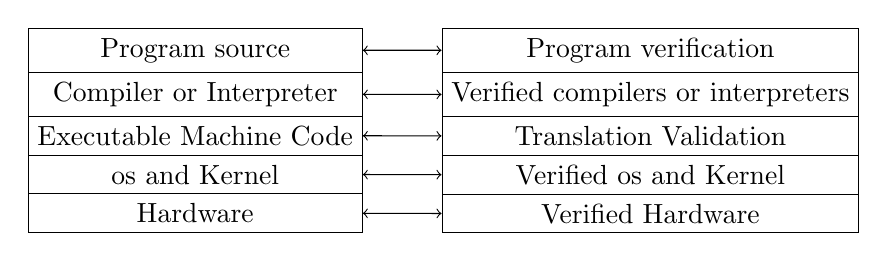
\begin{tikzpicture}[stack/.style={rectangle split, rectangle split parts=5, draw, anchor=center}]
        \node[stack](prog){%
            \nodepart{one}Program source
            \nodepart{two}Compiler or Interpreter
            \nodepart{three}Executable Machine Code
            \nodepart{four}\gls{os} and Kernel
            \nodepart{five}Hardware
        };
        \node[stack,right=of prog](verification){%
            \nodepart{one}Program verification
            \nodepart{two}Verified compilers or interpreters
            \nodepart{three}Translation Validation
            \nodepart{four}Verified \gls{os} and Kernel
            \nodepart{five}Verified Hardware
        };
        \draw[<->] (prog.one east) -- (verification.one west);
        \draw[<->] (prog.two east) -- (verification.two west);
        \draw[<->] (prog.three east) -- (verification.three west);
        \draw[<->] (prog.four east) -- (verification.four west);
        \draw[<->] (prog.five east) -- (verification.five west);
    \end{tikzpicture}
    \caption{A simplified programming environment and execution stack, with corresponding verification technology}\label{F:abstraction}
\end{figure}

The model presented in \figurename~\ref{F:abstraction} generally ignores
distributed systems and newer environments like the cloud; here we are primarily
concerned with a program running on a single machine, though it is possible to
generalize the model. We also ignore containerization, orchestration, and build
and deployment pipelines insofar as they are represented as user-space programs
or compositions thereof. Build pipelines naturally include compilers, which are
shown in the model despite being user-space programs.

Also out of scope is full-stack verification in the vein of
IronClad~\cite{hawblitzel2014ironclad} and
IronFleet~\cite{hawblitzel2015ironfleet}. Here we are considering the individual
components, especially the top layers.

At the very top of the stack, we have the program source. Whether high-level or
low-level, this is the definition of what we want the computer to do.
Verification requires a formal specification of that behavior and a proof that
the source-as-written, coupled with the language's formal semantics, implement
that behavior. This report focuses on tools and techniques for accomplishing
this task. Some key components include
\begin{inlist}
\item the kind of verifier (\eg, push-button or interactive);
\item the logic of the verifier (\eg, \gls{smt} or higher-order constructive
    propositional logic via \gls{coc}); and
\item the logical system of the proof (\eg, separation logic).
\end{inlist}

In order to execute the program, we have the remaining layers. In order:
\begin{enumerate}
    \item\label{i:stack_translator} A program translator (compiler or
        interpreter)\footnote{These are almost eschewed in the case of the
        assembly programmer; yet, there is still the assembler or linker to
        contend with.}
    \item\label{i:stack_asm} The produced executable machine code (\eg, ELF
        binaries)
    \item\label{i:stack_OS} The \gls{os} and kernel responsible for managing execution
        of the machine code
    \item\label{i:stack_hardware} The underlying hardware that carries out the
        instructions
\end{enumerate}

Item~\ref{i:stack_translator} produces executable machine code, possibly through
several stages of translation. In safety-critical systems, it is vital that
there be no mis-translation, \ie, bugs introduced by translation. Even outside
of such restrictive domains, it is important to trust that the translator
faithfully translates source code; otherwise, our systems are all subject to
vicious attack~\cite{Thompson_1984}. Thus a verified translator is an important
component in the software-development tool-chain. Verifying a translator amounts
to both a proof about a particular program---the translator itself---\emph{and}
a proof about a \emph{class} of programs---those accepted and generated by the
translator. A verified translator must preserve proofs about the source; that
is, if a program \(S\) is proven to have some property \(P\) (written \(S
\models P\) after~\cite{Leroy-Compcert-CACM}), translating with a verified
translator \(\func{Compiler}\) should imply that \(\func{Compiler}(S) \models
P\). Thus we have a statement about an entire class of programs, and it is this
type of statement that allows the composition of proven layers to be proven.

Item~\ref{i:stack_asm} is particularly interesting when the machine-code was
generated without a verified translator; in this case, the programmer has no
guarantees that the translation correctly and semantically matches the original.
This has generated much work on translation validation~\cite{Pnueli_1998}, which
proceeds by validating each run of a translator, comparing the executable code
to the source and guaranteeing that a \emph{particular} set of executable code
implements a \emph{particular} set of program source code. This stands in
contrast to verified-translator proofs, which need to cover an entire class of
programs. We will have only slightly more to say on this subject when we get to
verified translators; we point the interested reader to works such
as~\cite{Sewell:phd,Sewell_KH_16,Sewell_2013,Necula_2000}.

Items~\ref{i:stack_OS} and~\ref{i:stack_hardware} are out of scope for this
report. We refer the interested reader to research on verified \gls{os} and
kernels~\cite{Klein_EHACDEEKNSTW_09,Klein_AEHCDEEKNSTW_10,Klein_AEMSKH_14,Sewell_KH_16,Narayanan_2019,Narayan_2020,Nelson_2017}
and on verifying
processors~\cite{sturton-memocode13,Sturton_2013,Bradfield_2016,zhang2017identifying,zhang2018recursive,zhang2018end}.

\subsection{Structure of this report}

In Section~\ref{S:categories} we propose to classify the tools used to verify
programs. In Section~\ref{S:examples} we look at a few examples of verified
programs and identify a few prominent strategies and challenges. In
Section~\ref{S:discussion} we discuss the frontier of the formal-methods and
verified programs research, attempting to answer the question ``What are the
next big challenges to tackle for program verification?'' Finally, we conclude
with Section~\ref{S:conclusion}.


\section{Categorizing Verified-programming Tools}\label{S:categories}

I propose 3 axes along which to classify the tools used to verify programs.
These are
\begin{enumerate}
    \item the type of interaction;
    \item the type of proof logic; and
    \item the type of supported programming languages.
\end{enumerate}

I examine each in turn in Sections~\ref{S:t_interaction},~\ref{S:t_logic},
and~\ref{S:t_pl}.

One might also include the logic of the underlying verifier, especially in cases
where it differs from the proof logic. I choose not to because in the cases I
have studied they are the same (\eg, a Coq program proven in Coq~\cite{Coq}),
one is encoded in the other (\eg, a Dafny~\cite{leino2010dafny} program proven
by translation to Boogie~\cite{Barnett_2006,leino2008this}), or one is not
relevant to the other (\eg, proofs in Iris's logic~\cite{Jung_2018b} use Iris's
proof rules, while Iris is built on Coq). The programmer tasked with writing the
proof is concerned with the logic of the proof-system and the proof to be
written, except in the hopefully rare case of leaky
abstractions~\cite{Spolsky_2002}.

\subsection{Type of Interaction}\label{S:t_interaction}

\emph{TODO does \texttt{paragraph} or \texttt{subsubsection} work better?}

By ``interaction'' I mean that between the programmer and the verifier: what is
necessary to formulate proofs? Borrowing the terminology of~\cite[\S 2]{Nelson_2019},
I dissect this axis into 3 major types of interaction:
\begin{enumerate}
    \item Interactive,
    \item Auto-active, and
    \item Automatic (sometimes called ``push-button'').
\end{enumerate}

For each type the referenced~\cite{Nelson_2019} provides a plethora of further
examples.

\paragraph{Interactive verification.} This is the model employed by interactive
theorem-provers and proof-assistants such as Coq~\cite{Coq},
Isabelle~\cite{Isabelle}, and HOL~\cite{HOL}. The programmer, having written
programs and specifications, states theorems relating them (or lemmata,
corollaries, \etc, as the case may be). In order to prove the statements, the
programmer interacts directly with the system in a sort of call-and-response.
The verifier presents a goal: prove this statement. The programmer can execute
tactics to manipulate the goal, introduce quantified variables and hypothesis,
and otherwise make progress towards the proof of the goal. The verifier
represents the effect of these executions with another response, \eg, prove this
statement in this context. The programmer continues this dialogue with the
verifier, perhaps walking backwards and trying a different approach or walking
forwards through the steps of the proof, until the verifier has been given a
complete proof of all necessary goals.

Such systems may support automation in the sense of tactics that invoke other
tactics based on the goal or context; these can range from proof searches to
constraint solvers over linear integer arithmetic to manipulations necessary to
hide details of the underlying logical system.

\paragraph{Auto-active verification.} The approach taken by systems like
Dafny~\cite{leino2010dafny}. The programmer annotates code both with
specifications and proof hints, such as pre- or post- conditions or loop
invariants. The verifier translates the source into a verification condition and
uses a constraint solver to finish the verification. Some systems, such as
Dafny, permit annotations that rise nearly to the level of proof texts like
those of interactive verification, with composable theorems and lemmata in
addition to functional specifications and standard annotations. While writing
the proofs, though, the current state of the  goal and proof context are often
hidden or implicit, since they are being translated for the constraint
solver\footnote{The original goal and context are of course visible in the
original statement being proven.}. A call-and-response effort is possible in
such systems to complete a proof, but a major challenge is to discover what the
automatic part of the system cannot prove and actively provide effective hints
to make progress. One power of this type of system is to free the programmer
from all the details of the proof; the verifier often can handle simple
statements on its own, while more complex statements can be proven with only a
few well-directed hints. On the other hand, discovering which hints to use is
like a game of ``20 Questions''\footnote{The programmer asks ``Would you be
able to make progress on the proof if I could convince you of \(P\)?'' Based on
the verifier's response, which is essentially ``yes'' or ``no'', a sub-proof of
\(P\) is given through hints or not, and the game continues. The summer course
in~\cite{Kapritsos_2020} provides a detailed look at this style of proof in
Dafny.}, and the resulting proofs can be difficult to read.

\paragraph{Automatic verification.} The approach taken by
Rosette~\cite{Torlak_2013}. An automatic verifier restricts the class of
properties and programs that be verified in order to fully automate the process.
The essential limit is finitization: finite specifications that can be
implemented without unbounded loops allows symbolic evaluation or execution to
generate constraints that can be handed off to a solver, much like in
auto-active verification. The developer thus programs in such a restricted
system and pushes the ``verify button'', invoking the symbolic evaluator and
constraint solver. The limitations allow a greater degree of automation than in
the previous cases, leading to the descriptor ``push-button verification''---no
proof annotations are necessary. Such systems have been used to build
surprisingly sophisticated programs given the finitization requirement; examples
include the Yggdrasil file-system~\cite{Sigurbjarnarson_2016} and the
Hyperkernel OS~\cite{Nelson_2017}.

A related challenge is exponential path explosion: symbolic evaluation may have
to consider a rapidly-growing number of symbolic paths while generating
constraints. Rosette takes steps to solve this via aggressive partial
evaluation~\cite{Torlak_2013,Torlak_2014}, lenient symbolic
execution~\cite{Chang_2018}, and
profiling~\cite{Bornholt_2018,Porncharoenwase_2020}. Also related, as in the
case of auto-active verification, is the challenge of communicating back to the
developer the meaning of the results in the program domain.

\subsection{Type of Proof Logic}\label{S:t_logic}

A full account of proof-logics for programs would be a long paper in its own
right and is out of scope for this report. Look no further than
\figurename~\ref{F:iris_complex} to see how complicated the topology of (a
subset of) proof-logics can be. Instead, I will mention a key proof-logic
(namely, Hoare logic) and some of its extensions. For another mention of
program- and proof- logics and their uses, see~\cite[\S 5]{Appel_2011}.

\begin{figure}
    \centering
    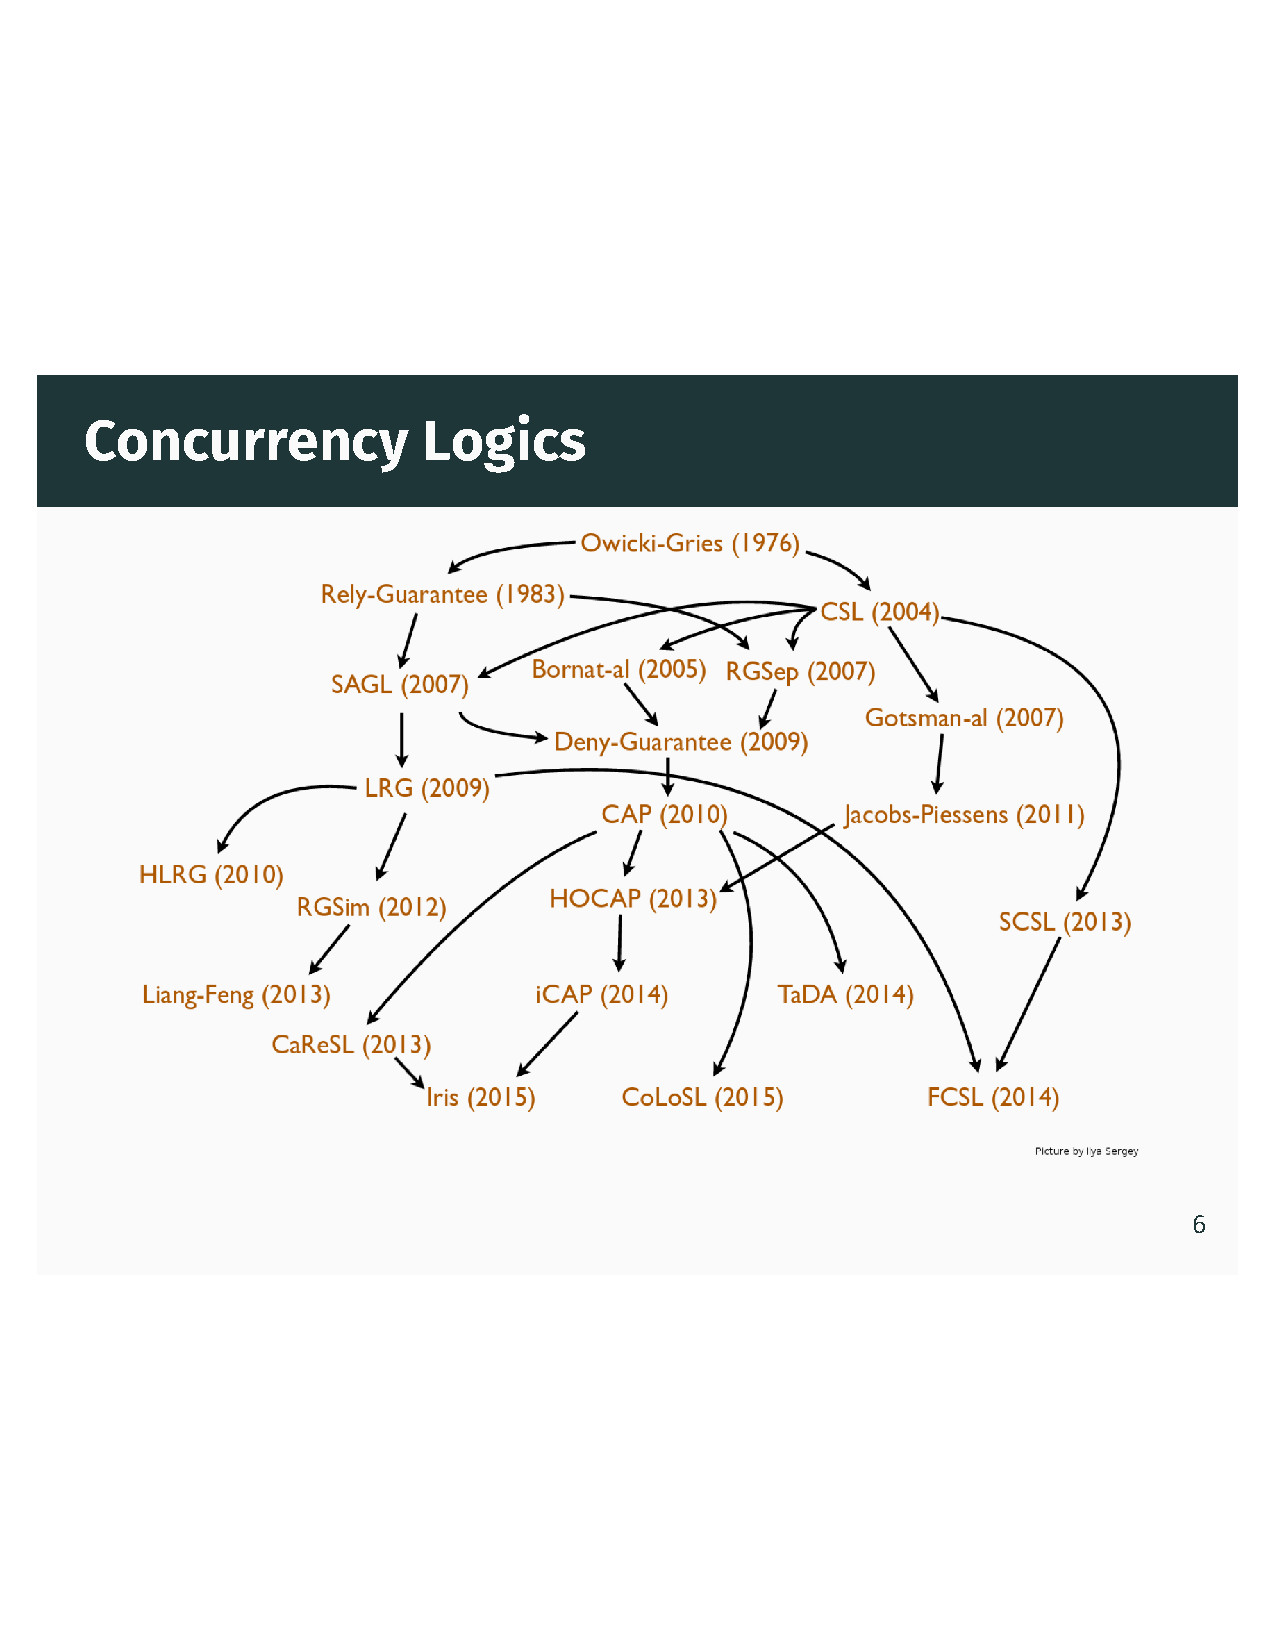
\includegraphics[width=\textwidth]{img/iris_2_0_concurrent_logics}
    \caption{A figure from a presentation on Iris~\cite{Jung_2016_slides}
    depicting the relationship of many concurrent separation logics developed
    specially for a system or proof. Iris notably attempts to distill these
    logics to their core, providing a system inside of which any of the
    individual logics may be derived.}\label{F:iris_complex}
\end{figure}

All proof-logics for programs combine a set of logic-rules with the semantics of
the program's language. In the simplest case, the programmer combines
``regular'' logic (in the sense of \gls{coc} or ZFC) with the semantics to write
proofs about program equivalences, termination, and transformations.
\emph{Software Foundations} shows it's possible to prove interesting
meta-theoretic\footnote{``meta'' because they are ``properties of the language
as a whole, rather than of particular programs''~\cite{Pierce:SF2}. It is also
possible to prove claims about specific programs this way, but, at least in some
systems, this becomes unwieldy.} claims about a language using these techniques
in their discussions about \emph{Simple Imperative Programs}~\cite{Pierce:SF1}
and \emph{Program Equivalence}~\cite{Pierce:SF2} and provides an introduction to
such proofs. Essentially, standard reasoning rules about logic formulae are
combined with the inference rules that define the semantics. An example is
provided in \figurename~\ref{F:Imp_ex}. I refer
to~\cite{Winskel_1993,Harper_2016} for introductions to program semantics.

\begin{figure}
    \centering
    \begin{tabular}{c}
        E-APlus \\
        \(e_1 \to n_1\) \quad \(e_2 \to n_2\) \\
        \midrule
        \(e_1 +_e e_2 \to n_1 + n_2\) \\

        \\

        E-Seq \\
        \((c_1, s_1) \To s_2\) \quad \((c_2, s_2) \To s_3\) \\
        \midrule
        \((c_1;c_2, s_1) \To s_3\)
    \end{tabular}
    \caption{Sample inference rules for \texttt{Imp}, a simple imperative
    language. E-APlus shows how to add two arithmetic expressions, where \(\to\)
    means ``evaluates to.'' Similarly, E-Seq shows how to sequence two
    statements \(c_1, c_2\), where \((c, s)\) represents a pair of a statement
    and a state and \((c, s) \To s'\) means ``evaluating statement \(c\) in
    state \(s\) produces the new state \(s'\).''}\label{F:Imp_ex}
\end{figure}

\subsubsection{Hoare Logic}

When turning to program verification\footnote{Recall \citeauthor{EWD:EWD1036}'s
act of proving a program implements its specification.}, \emph{Software
Foundations} introduces Hoare logic. Hoare logic, with its many variations, is
the predominant proof-logic for program verification. Originating in
\citeyear{Hoare_1969} with \citeauthor{Hoare_1969}'s paper~\cite{Hoare_1969},
Hoare logic formalizes the notion of pre- and post-conditions with the
\emph{Hoare triple}, written

\begin{equation*}
    \{P\} C \{Q\},
\end{equation*}

to indicate that command \(C\) has pre-condition \(P\) and post-condition
\(Q\), both assertions (\eg, a claim about the current state). If \(P\) is
established, executing \(C\) establishes \(Q\) (or \(C\) diverges). The
programmer indicates that \(C\) diverges in a Hoare triple by choosing \(Q =
\bot\). Hoare logic permits reasoning about partial correctness; termination
must be proven separately\footnote{Various sources claim it is possible to give
rules for total correctness.}. The statement of the triple can thus be written
using notation from \figurename~\ref{F:Imp_ex}, and assuming \(P\) and \(Q\) are
functions from states to propositions

\begin{align*}
    \{P\} C \{Q\} \definedas \forall s, s' : &(C, s) \To s' &\text{if \(C\) terminates} \\
    &\implies P s &\text{and if \(P s\) holds} \\
    &\implies Q s' &\text{then we can establish \(Q s'\) holds.}
\end{align*}

This is a model-theoretic Hoare logic: the proof-rules are stated in the terms
of the model. Hoare logic can also be defined in proof-theory; this is arguably
more common~\cite[Ch. \emph{Hoare Logic as a Logic}]{Pierce:SF2}. Such a
statement avoids ascribing direct meaning to Hoare triples and instead gives
syntactic derivation rules. These rules are the same judgements as in the
model-theoretic definition, and the two are consistent with each other.

Reasoning with Hoare logic mimics the structure of the program,
as triples can be effectively combined to build up claims about the entire
program. The rules for doing so resemble those of ``regular'' logic formulae
above, with some connectives for strengthening pre-conditions or weakening
post-conditions. Formalizations and uses of these rules often work backwards;
the natural way to construct a Hoare logic proof is to start at the final
post-condition and move backwards to the beginning. A selection of rules are
presented in \figurename~\ref{F:Hoare_ex}.

\begin{figure}
    \centering
    \begin{tabular}{c}
        Hoare-Consequence-Pre \\
        \(\{P'\} C \{Q\}\) \quad \(P \TO P'\) \\
        \midrule
        \(\{P\} C \{Q\}\) \\

        \\

        Hoare-Seq \\
        \(\{P\} C_1 \{Q\}\) \quad \(\{Q\} C_2 \{R\}\) \\
        \midrule
        \(\{P\} C_1;C_2 \{R\}\)
    \end{tabular}
    \caption{Two examples of the rules of Hoare logic. Hoare-Consequence-Pre
    captures the notion that we can strengthen the pre-condition from \(P'\) to
    \(P\) and still have a valid triple (\(\TO\) is analogous to implication,
    with the definition \(\forall s: P s \implies P' s\)). Hoare-Seq provides an
    analogue to E-Seq from \figurename~\ref{F:Imp_ex}. The programmer composes
    rules like these rather than invoking the definition of a Hoare triple
    whenever possible, using a higher level of abstraction.}\label{F:Hoare_ex}
\end{figure}

I should note that Hoare logics are mostly seen for imperative programming
languages. (\emph{TODO what about functional languages? Rust is nearly
functional, but \(\lambda_{\text{Rust}}\) from RustBelt uses a CPS-style
\(\lambda\)-calculus combined with CSL in Iris?})

\subsubsection{Pre-, post-, and weakest conditions}

The choice of pre- and post- conditions is up to the programmer, who wants to
prove that the program implements a spec \(\var{Spec}\). A natural choice for
the post-condition is some \(Q\) that implies \(\var{Spec}\). Similarly, a
natural choice for the pre-condition is some \(P\), possibly corresponding to
constraints on the program inputs, and that also allows the programmer to prove
\(\{P\} C \{Q\}\). Then we can claim that if \(C\) terminates under
pre-conditions \(P\) then \(P \implies C \models \var{Spec}\).

The programmer could also choose \(P = \bot\), in which case any post-condition
at all is valid, including the \(Q\) that entails \(\var{Spec}\) from earlier
(check the definition of the triple, and observe that this is a case of the
principle of explosion). But this ridiculous pre-condition is never satisfied,
so in practice we have proven nothing about \(C\), except that if it terminates
any behavior whatsoever is allowed!

In a similar vein, we can always add extraneous information to the pre-condition
which is not used; this does not necessarily invalidate our proof in the same
way, but such information may not be needed.

To prevent such absurd pre-conditions as \(\bot\) and to streamline their
generation, many systems make use of ``weakest
pre-conditions''~\cite{dijkstra1976discipline,Nelson_1989} (cited
in~\cite{leino2008specification}). The intuitive idea is that for some statement
\(C\) and some post-condition \(Q\) we denote by \(\wpre{C, Q}\) the ``minimal''
information we need to correctly establish \(Q\), \ie, such that the triple
\(\{\wpre{C,Q}\} C \{Q\}\) is provable. The programmer must still choose an
appropriate \(Q\) to establish \(\var{Spec}\); the generation of the required
pre-conditions can now be automated. Note that this does not mean the proof will
be straightforward with \emph{only} these pre-conditions! The programmer may
need to make logical leaps to strengthen conditions as necessary, particularly
where complex algebraic reasoning is required.

Formally, \(P\) is a weakest pre-condition with respect to \(C\) and \(Q\) iff
\begin{equation*}
    \{P\} C \{Q\} \text{ and } \forall P', \{P'\} C \{Q\} \implies (P' \TO P).
\end{equation*}

The function \(\func{wp}\) is computable by structural induction on
\(C\). Crucially, it is not a decidability function; it returns a proposition,
not a proof. An extended example is found in~\cite[\S 3]{leino2008specification},
where weakest pre-conditions provide the vehicle used to translate from
Dafny~\cite{leino2010dafny} to Boogie~\cite{Barnett_2006,leino2008this}.

\subsubsection{Separation Logic}

According to~\cite[\S 5]{Appel_2011}, ``Ordinary Hoare logics have difficulty
with pointers and arrays, especially with updates of fields and array slots.''
To solve this problem, \citeauthor{Reynolds} invented \emph{separation
logic}~\cite{Reynolds}.

The crucial extension is to differentiate between the assertion \(P \land Q\),
which denotes that both conjuncts hold on the current state, and the assertion
\(P * Q\), which denotes that each conjunct holds on a disjoint part of the
current state. In other words, the state \(s\) can be split into \(s_1, s_2\)
(often written \(s = s_1 \uplus s_2\)) such that \(P\) holds on \(s_1\) and
\(Q\) holds on \(s_2\). Along with rules for manipulating this new separating
conjunction, the programmer gains the ability to reason about separate parts of
the store or state.

Other important rules in separation logics correspond to framing (as in
``framing the world'', not ``stack frames'') and address and pointer manipulation.

\subsubsection{Concurrent Separation Logic}

For reasoning about concurrency, Hoare logic and separation logic remained
inadequate; \citeauthor{O_Hearn_2007} proposed a \emph{concurrent separation
logic} to solve the problem~\cite{O_Hearn_2007}. \citeauthor{Brookes_2007}
provides a model in the companion paper~\cite{Brookes_2007}. Both papers discuss
the difficulty of soundness in such a logic---that, and the plethora of
subsequent separation and concurrent logics that have been developed
(\figurename~\ref{F:iris_complex}), each with their own complex rules,
demonstrate the difficulty both of developing and reasoning in a concurrent
separation logic. Reasoning about parallel programs may bring inherent
complexity to the problem. The various concurrent logics add rules required for
their specific uses, \eg, partial ownership or permissions in the case
of~\cite{Appel_2011}, which might require use of a separation algebra. Iris
carries these constructions to their limits, developing a foundational
separation algebra and parameterized logic that can be used to derive new
logics~\cite{Jung_2018b}.

One of the original concurrent separation logic proof rules
from~\cite{O_Hearn_2007} is presented in \figurename~\ref{F:CSL_ex}.

\begin{figure}
    \centering
    \begin{tabular}{c}
        \(\{P_1\} C_1 \{Q_1\}\) \quad \(\{P_2\} C_2 \{Q_2\}\) \\
        \midrule
        \(\{P_1 * P_2\} C_1 \parallel C_2 \{Q_1 * Q_2\}\)
    \end{tabular}
    \caption{A separation logic rule for reasoning about the concurrent
    execution of \(C_1\) and \(C_2\), denoted by \(\cdot \parallel \cdot\)
    from~\cite{O_Hearn_2007}.}\label{F:CSL_ex}
\end{figure}

\subsection{Type of Supported Programming Languages}\label{S:t_pl}

The supported languages are as varied as the programming language options
available to today's programmer, from MLs~\cite{Coq,Kumar_2014}, Lisps and
Schemes~\cite{Torlak_2013} to object-oriented
systems~\cite{leino2008specification,leino2010dafny} and bare-metal
assembly~\cite{Chlipala_2011} on top of which further abstractions can be
built~\cite{Chlipala_2015}. While this variety appears to present overwhelming
choice to the programmer who wishes to verify a program, reality belies a
simpler problem: some languages and design decisions are better suited to
certain problem domains than others. Correspondingly, certain proof logics are
better suited to certain domains, and one often finds pairings between language
and logic for the task at hand.

I recommend a few starting points for programmers seeking a particular language
style for their problems and discuss options available to those unsatisfied with
the existing languages.

The systems programmer is apt to look more towards C and Rust like systems; this
lends itself to a choice of tools like Bedrock~\cite{Chlipala_2011},
\gls{vst}~\cite{VST}, and CompCert~\cite{Kastner-LBSSF-2017}, possibly paired
with (concurrent) separation logic. Ynot~\cite{Nanevski08ynot:reasoning} is also
an option for those comfortable with monadic reasoning and Hoare logic.

Programmers in ML-like languages have Coq~\cite{Coq}, CakeML~\cite{Kumar_2014},
and similar tools to choose from; Lispers and Schemers look to both
relational-logic systems like Kanren~\cite{Byrd_2009} and automatic verifiers
like Rosette~\cite{Rosette}.

For the unsatisfied, Rosette promises the ability to build automatic
solver-aided languages suited to the problem at hand~\cite{Torlak_2013}. For
those seeking an auto-active style, the discussion
in~\cite{leino2008specification} offers a design for an object-oriented language
that could be adapted. When building a for a completely interactive environment,
building on top of existing systems is the norm. It is always possible to build
a compiler\footnote{or \emph{transpiler}, as some prefer} targeting a
higher-level verified language---the programmer thus has complete control of the
surface language, at the cost of building, maintaining, and perhaps verifying a
compiler. The ease of such an effort depends on how well the languages semantics
match; syntax is a matter of appropriate translation.

% \input{applications}
% \section{Discussion}\label{S:discussion}

Having given an overview on verified programming and the tools used to build
verified programming languages, I turn now to the frontier of the science: what
challenges lie ahead? What open problems need answers?

We saw in Section~\ref{S:stack} that today's programming environment is more
expansive than a single program on a single machine.
IronClad~\cite{hawblitzel2014ironclad} and
IronFleet~\cite{hawblitzel2015ironfleet} address full-stack distributed
verification, but I have not found any research on build-pipeline or deployment
verification, nor on containerization, orchestration, and the like. On the one
hand, we might hope that deployment steps are simple enough that the
cost-benefit ratio of formal verification indicates the effort is not worth the
confidence. Yet the mishaps that occur on mis-deployment might indicate
otherwise, and the complexity of rollouts for some teams indicate a need for
increased confidence. With respect to a build-pipeline, verified compilers like
CompCert~\cite{Kastner-LBSSF-2017} yield verified compilation stages, but there
are often other steps before and after compilation that are left unverified
(they may, of course, be tested). There may be room to grow in this direction as
well. Lastly, verified containerization technology would improve on today's
state of systems based on Docker~\cite{merkel2014docker} and
Kubernetes~\cite{k8s} by being able to guarantee the security and isolation
promises of containerization, just like RustBelt~\cite{Jung_2018a} is now able
to guarantee the safety promises of Rust.

In the same section, we peeked into the deeper layers, like the executable
machine code, the \gls{os}, and the hardware. Translation
validation~\cite{Pnueli_1998} and verified compilers give confidence in the
machine code, but CompCert still lacks a fully verified assembler and linker. A
number of projects are researching verified \gls{os} and kernels (see
Section~\ref{S:background} for a list) and discovering their own unique
challenges in design and proof-management~\cite{Klein_AEMSKH_14}. Hardware
presents verification challenges different from those of software; some current
research is examining security properties and symbolic execution \`{a} la
Rosette for hardware~\cite{zhang2018end}.

In Section~\ref{S:t_interaction} we saw 3 types of verification tools
(interactive, auto-active, and automatic) and examples of proofs in each. In our
examples from Section~\ref{S:ex_ext}, we saw a comparison between one
interactive proof and one auto-active proof, where both had benefits. Tools like
Rosette and other push-button approaches bring more automation, at certain
costs (\eg, finitization). Developing better automation tools for the
interactive provers (\eg, Mtac~\cite{Kaiser_2018}, Iris proof
mode~\cite{Krebbers_2017b}) will bring them closer to push-button tools, making
them more accessible to an average developer. On the other hand, developing
tools that provide more robust insights to the automatic provers (\eg,
profiling~\cite{Bornholt_2018,Porncharoenwase_2020}) can help the programmer
solve automation-related problems, especially exponential path explosion, scale,
and timeout-demons. In a related vein, we saw the use of \texttt{\{:opaque\}} to
combat automation issues related to quantifiers, and we also saw that Coq
struggles to rewrite under the existential quantifier, demonstrating needs for
improvements on these facets of the system.

Iris and Section~\ref{S:t_logic} demonstrated that proof logics (\eg, extensions
to Hoare-logic) are still under active development: although systems often need
to build their own proof logics, checking that they are sound is a difficult
process. Further, explaining and using them requires deep background. What new
proof logics will we need to keep up with the state of programming technology?
Iris was developed in part specifically for Rust; it also managed to position
itself as a foundation for several older, more complex proof logics. As our
language technology evolves, we will need increasingly sophisticated logics. We
also hope to keep them accessible to the programmer writing proofs. Another
possible direction here is to enable more rapid proof development: when
developing a language model for a proof, like Rust, the programmer has to tie
the syntax, semantics, and proof logic together. Facilitating these steps would
help automate early development and allow the programmer to focus more on the
proofs of interest. It would also enable a tighter feedback loop between model
changes and proof updates.

Section~\ref{S:t_pl} mentions several programming languages or paradigms along
with their accompanying verification tools. Bringing verification to more
languages and more languages to verification will remain an open problem for as
long as we continue to develop new programming languages. One technique for
verifying new languages is to lift a non-verified language into an
already-verified language~\cite{leino2008specification}. A particular challenge
when modelling new languages is to verify that the model is accurate to the
language specification and implementation; CompCert provides a reference
interpreter~\cite{Kastner-LBSSF-2017} for that purpose, though doing so is
challenging~\cite[Chs.\ \emph{Simple Imperative Programs}, \emph{An Evaluation
Function for Imp}]{Pierce:SF1}. In a similar vein, verifying compilation or
interpretation for more languages would bring increased confidence to systems
using those languages. Although avionics is one example of safety-critical
applications that relies on formal techniques, applications like financial
software may not use them to their full extent, in part due to a lack of
appropriate technology.

When we looked at the extended examples in Section~\ref{S:ex_ext}, we saw early
on that some programs and proofs produce executable programs, while others are
only models that cannot actually be run. Proof by refinement can later tie an
executable to the model, but refinement is often a meta-technique: there is no
built-in support for the technique, so the programmer must build out both the
technique and the argument that it is applicable. Similarly, the inductive
state-machine model is better supported by some languages (\eg, Coq's inductive
types) than others (\eg, Dafny's relation predicates, which are not tied
together by any meaning other than what the programmer ascribes), which also
impacts the statement of the specification. We also saw that graph and
bit-vector proofs are unwieldy in some languages~\cite{Morrisett_2012}.

We do see in the extended examples one use of parametric or abstract modules;
Iris takes a similar approach, allowing the programmer to instantiate the module
with specifics of the problem. The concept comes from ML's module system;
specifically, it is analogous to functors in ML and OCaml, which are
module-level functions from modules to modules. Developing further abstraction
mechanisms might prove fruitful for some of the problems of proof development
and automation.

Other research demonstrated open problems in various related fields. For
example, RockSalt~\cite{Morrisett_2012} shows a lack of strong tooling for
assembly-language semantics and related verification. Their DSL development
takes promising steps towards improving the state of assembly verification. It
also exposed questions of scale, portability, and testing (see
Section~\ref{S:ex_notable}). Rosette identified challenges related to symbolic
path explosion~\cite{Bornholt_2018,Porncharoenwase_2020}. CompCert exposes the
problems of verifying linkers and assemblers in addition to questioning the
extraction mechanism. Bootstrapping verified compilers is a studied but
non-trivial technique~\cite{Konat_2016,Myreen_2021}, and the goal for CompCert
is to extract verifiable C from the Coq development. Jitterbug~\cite{258848}
raises questions about integrating proof-developments into live software like
the Linux kernel, where a clean-slate approach is impossible. They also
reinforce the challenge of symbolic execution. One facet of the Jitterbug
development involved reasoning across different verifiers (in particular,
interactive and automatic), an area which has seen little research to my
knowledge. Serval examined the challenge of separating implementation and
verification while maintaining the necessary connections~\cite{Nelson_2019}.
Bedrock, in a vein similar to Serval and CompCert, took one of the first looks
at cross-language verification~\cite{Wang_2014}.


\glsresetall[acronym]

% \section{Conclusion}

\subsection{Further work}


\begin{singlespace}
    \newpage
    {\printbibliography[heading=bibintoc]}

    \newpage
    \printglossary[title={Abbreviations},type=acronym,style=long]
\end{singlespace}

\end{document}
